\documentclass[a4paper,10pt, sans]{article}
\usepackage[utf8x]{inputenc}
\usepackage[spanish]{babel}
\usepackage{hyperref}
\usepackage{verbatim}
\usepackage{graphicx}
\usepackage{float}
\usepackage{wrapfig}
\usepackage{ltxtable}
%\usepackage{amsmath,amssymb,amsfonts,latexsym,cancel}
\usepackage{multicol}      %para usar varias columnas
  %uso:
  %\begin{multicols}{2}
    %texto
  %\end{multicols}
\usepackage{marvosym}

\setlength{\columnsep}{4mm}    %separación de columnas
%\usepackage{pslatex}
%\hoffset -0.75in        %cambio el margen horizontal izquierdo
%\voffset -0.9in          %cambio el margen vertical superior
\textwidth 17cm        %ancho de texto. defaut: 14cm
\textheight 25cm        %alto de texto. default: 19cm
\topmargin -1cm        %agranda el margen superior. default: 3cm
\oddsidemargin -1cm        %agranda el margen izquierdo. default: 2.5cm (4.5 si no aparece esta instrucción)
\pagestyle{empty} %{myheadins}  %numeración de pág: sin / arriba
\parskip 2mm          %X mm entre párrafos
%\parindent 0mm          %elimina sangría

\begin{document}
  

\begin{wrapfigure}{r}{4cm}
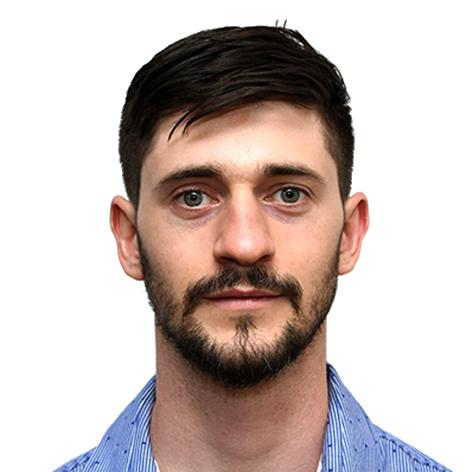
\includegraphics[height=4cm]{seba_4x4.jpg}
\end{wrapfigure}

\sffamily

\begin{Huge}
Sebastián Rossi
\end{Huge}
\\ \\
\hspace*{0.5cm} \textit{CURRICULUM VITAE} \\
\hspace*{0.5cm} {\textit{Updated: 02/02/2024}}

\begin{tabular}{rl}
\vspace{0.5cm} \\
\large\Mobilefone & \textbf{+549 3402 507471} \\
\large\Letter & \textbf{srossi@inti.gob.ar} \\
{}            & \textbf{sbstnrossi@outlook.com}
\end{tabular}

\vspace{0.5cm}
\large
\begin{table}[H]
  \begin{tabularx}{\textwidth}{r X}
    %%%%%%%%%%%%%%%%%%%%%%%%%%%%%%%%%%%%%%%%%%%%%%%%%%%%%%%%%%%%%%%%%%%%%%%%%%%%
    \textbf{Personal} & {} \\ [1ex]
    \textbf{Details} & Birth date: 15-11-1988 \\ [1ex]
      {} & Nationality: Argentinian - Italian \\ [1ex]
      {} & Address: Maipú 782, (2107) Álvarez, Santa Fe, Argentina \\ \\ \hline \\

    \textbf{Education} & {} \\ [1ex]
       (2020 - ) & \textbf{Doctorado en Ingeniería (Doctor of Engineering)}, FCEIA, Universidad Nacional de Rosario (UNR). Thesis: Sensing and control of pneumatic planting systems. Supervisors: Ignacio Rubio Scola, Gastón Bourges.\\ [1ex]
       (2008 - 2014) & \textbf{Ingeniero Electrónico (Electronic Engineer)}. FCEIA, UNR.\\ \\ \hline \\


    
    
    \textbf{Employment} & {}\\ [1ex]
      (2013 - ) & Instituto Nacional de Tecnología Industrial (INTI - National Institute of Industrial Technology). Department of Industrial Products Engineering - Rosario.\\ \\
            
        {} & \hspace{2cm} \textit{Development of new capabilities.} \\ [1ex]
        
        (2013) & Temperature distribution and thermal stabilization time measurements in gauge blocks calibration laboratory to determine their effects on the reported uncertainty. \\ [1ex]
        (2013 - 2014) & Software development for data acquisition by serial port of a gauge block comparator. Programmed in Python.\\ [1ex]
        (2014 - 2015) & Development and implementation of a multichannel recording system commanded by Wi-Fi with Raspberry Pi boards. Application: Seed impact detection. \\ [1ex]
        (2015) & Scilab script development for determining impact times of different kinds of seeds from piezoelectric sensor signal and seed metering systems evaluation according to ISO 7256. \\ [1ex]
        (2016) & Cortex M4 based platform programming for synchronized multi channel piezoelectric sensors for seed impact detection. Programmed in C.\\ [1ex]
        (2016 - 2017) & Documentation drafting to integrate the strain gauge measurement service into the quality management system. \\ [1ex]
        (2017 - 2019) & Air-drill system test bench experimentation for different levels of air speed, seed density, distributor head configuration and exit pipe lengths with soybean seeds. \\ [1ex]
        (2018) & Cortex M0 based modular platform development with wireless communication for data acquisition of multi channel piezoelectric sensors and pressure transmitters. Programmed in C. Two layers PCBs designed with Altium.\\ [1ex]
        (2019 - 2020) & Image processing software development in python using OpenCV library for seed trajectory detection in high frame rate videos for evaluating seed meters and seed delivery tubes in a test bench over a shaker. R script for results analysis. \\ [1ex]
        (2020 - 2021) & Static bench experiment for uncertainty evaluation of seed and trajectory detection systems with impact plate and image processing. \\ [1ex]        
        (2022 - 2023) & Static bench experiment for uncertainty evaluation of seed detection systems with different materials of impact plate and infrared sensor array. \\ [1ex]  
        (2023 - ) & 2 axes optic sensor array for seed pass detection. Cheap thresholding electronic circuitry that follows CC component. Detection method running in ESP32 Dev kit board.\\
  \end{tabularx}
  \end{table}



  
  \begin{table}[H]
  \centering
  \begin{tabularx}{\textwidth}{r X}  
  		
        {} & \hspace{2cm} \textit{Work done for clients.} \\ [1ex]
        (2015 - 2016) & Evaluation of an in-line seed drill using piezoelectric sensors both in test bench and in field (soybean) based on ISO 7256 Part 2. Client: Indecar. \\  [1ex]

        (2015 - ) & Evaluation of precision seed meters and seed delivery tubes with image processing and piezoelectric sensors based on ISO 7256 Part 1, both in static and dynamic (shaker) test benches. Clients: Agrometal, Pla, Siembra Neumática. \\ [1ex]
        (2016 - ) & Bonding of strain gauges and measurement of deformations in steel structures. Clients: Acerías 4C, Agrometal, Crucianelli, Ejército Argentino, Hermann, Juri, Ombú, Palfinger, Pla, Randon, Sola y Brusa, Superwalter. \\ 
        (2023 - ) & Technology transfer for seed pass detection in static test bench for in factory seed meter evaluation. Client: Siembra Neumática.\\ \\ \hline \\




    \textbf{Publications} & {}\\ [1ex]
      {Journals} & {Rossi, S., Rubio Scola, I., Bourges, G., Sarauskis, E., Karayel, D. (2023) \textit{Improving the seed detection accuracy of piezoelectric impact sensors for
precision seeders. Part I: A comparative study of signal processing algorithms}. Computers and Electronics in Agriculture. Vol 215. 108449.} \\ [1ex]
      {} & {Rossi, S., Rubio Scola, I., Bourges, G., Sarauskis, E., Karayel, D. (2023) \textit{Improving the seed detection accuracy of piezoelectric impact sensors for precision seeders. Part II: Evaluation of different plate materials}. Computers and Electronics in Agriculture. Vol 215. 108448.} \\ 
      {Book chapters} & {Rubio Scola, I., Rossi, S., Bourges, G. \textit{Air drill Seeder Distributor Head Evaluation: A Comparison between Laboratory Tests and Computational Fluid Dynamics
Simulations}. Chapter of book: \textit{Information and Communication Technologies for Agriculture — Theme II: Data}.} \\
      {Conference papers} & Bourges, G., Rossi, S., Eliach, J., Medina, M. \textit{Experimental evaluation of a precision seed meter.} (in Spanish) V CAIM 2016. Santiago del Estero, Argentina. UNSE- FCEyT- ISBN: 978-987-1676-63-7. pp: 881-891. \\  [1ex]
      {} & \textit{Tests on a precision seed meter.} (in Spanish) X Jornadas de Ciencia y Tecnología. Sede de Gobierno. UNR. Rosario, Santa Fe. \\  [1ex]
      {} & Rossi, S., Rubio Scola, I., Eliach, J., Bourges, G. \textit{Performance evaluation of a precision seed meter by means of filming and image processing.} (in Spanish) VII CAIM 2020. San Nicolás, Argentina. \\  [1ex]
      {} & Bourges, G., Rossi, S., Rubio Scola, I., Karayel, D. \textit{Incidence evaluation of different factors in the distribution of soybean seeds in a pneumatic transport system.} (in Spanish)  VII CAIM 2020. San Nicolás, Argentina.  \\  [1ex]
      {} & {Rossi, S., Rubio Scola, I., Bourges, G., Eliach, J., Šarauskis, E., Karayel, D. \textit{Improving seed detection accuracy with infrared sensors array in precision seeders}. VIII CAIM 2023. Santa Fe, Argentina.} \\ \\ \hline \\
    
    
    
    
    \textbf{Courses} & {}\\ [1ex]
    {} & Measurement uncertainty evaluation. 16 hs. INTI Rosario. \\  [1ex]
    {} & Solidworks. 24 hs. Disegno Soft S.R.L. \\  [1ex]
    {} & PIC microcontrollers programming in C language. 30 hs. Postgraduate school of FCEIA, UNR. \\  [1ex]
    {} & Digital systems synthesis in FPGA. 30 hs. Postgraduate school of FCEIA, UNR. \\  [1ex]
    {} & RTOS on 32 bits based microcontrollers. 30 hs. Postgraduate school of FCEIA, UNR. \\  [1ex]
    {} & Experiment design. 30 hs. Postgraduate school of FCAgr, UNR. \\  [1ex]
    {} & Multivariate analysis. 50 hs. Postgraduate school of FCAgr, UNR. \\  [1ex]
    {} & Introduction to design and analysis of industrial experiments. Graduate school of FCECON, UNR. \\  [1ex]
    {} & Digital Image Processing. 70 hs. Postgraduate school of FCEIA, UNR. \\  [1ex]
    {} & Modelling and simulation of dynamic systems. 70 hs. Postgraduate school of FCEIA, UNR. \\ \\   
    
  \end{tabularx}
  \end{table}



  
  \begin{table}[H]
  \centering
  \begin{tabularx}{\textwidth}{r X}  
    
    \hline \\  
    \textbf{Languages} & {} \\ [1ex]
    {} & Spanish, native language. \\ [1ex]
    {} & English, intermediate level. \\ \\ \hline \\
      
    \textbf{Driver's license} & {} \\ [1ex]
    {} & Argentinian, A3 and B2 classes.\\
    
  \vspace{5cm}
  \end{tabularx}
  \end{table}
  
\end{document}
